\documentclass[main]{subfiles}


\begin{document}
\newpage
\section{Plasticity In The Brain}

%---------------------------
\subsection{Why do we need plasticity?}
Why this topic is relevant:
\begin{itemize}
    \item Biological plasticity might provide a different angle to understand the training procedures in DNNs.
    \item Given the effectiveness of human brain learning bio-plasticity might provide inspiration/new ideas for improved DNN training algorithms. Example: the idea of drop out (in DNNs the network randomly get rid of single neurons to prevent too much information to be stored in single neurons and weights. This was observed in neuroscience first)
    \item Understanding biological plasticity might help to better understand how (hierarchical) learning is organized in the brain (Learning and Memory).
    \item Many neural disorders such as dementia might relate to a disturbance in neuronal plasticity that cause neuronal networks to become dysfunctional. Some plasticity mechanisms /disorders lead to malfunction in the brain.
    \item All intelligent behavior is learned so we need plasticity to learn. 
    \item The brain a universal learning machine, some information is genetically present at birth such as babies ability to distinguish faces but the rest is learned thus requires plasticity. 
\end{itemize}
\begin{itemize}
    \item[\textbf{Plasticity}] Allows acquisition of knowledge/information and the formation of memory through experience
    \item[\textbf{Memory}] Storage of information that can be recalled later. Learning results in memory - which has further outcome - it can change future behavior
    \item[\textbf{Learning Curve}] Training to do tasks or reacting to stimuli, at the beginning bad and over the course of a few days vastly improves
\end{itemize}
%
Everything we do is \textit{learning} and for that we need \textit{plasticity}. An illustrative example below\footnote{Kandel, \textit{Principles of neural science}, 2001}, according to the motto: "Here I get a reward, here not".
%
\begin{figure}[H]
    \centering
    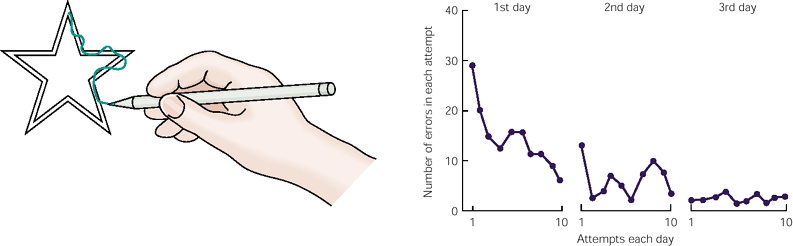
\includegraphics[width=\textwidth]{03_PlasticityInTheBrain/figures/motorlearning.jpg}
    \caption{Motor learning task. Some human subjects have got the task to draw. Having gotten an (electrical) feedback, this subjects learned the pattern they had to draw}
    \label{fig:motorlearning}
\end{figure}

%---------------------------
\subsection{Synaptic Plasticity}

\subsubsection{Biological Recap}
In synaptic plasticity one understands changes in reactivity of \textbf{post}- to \textbf{pre}synaptic neuron. In other words, plasticity changes of chemical synapses can strengthen or weaken transmission. This changes can last from milliseconds (short-term) to weeks or longer (long-term).
\begin{itemize}
    \item[\textbf{EPSP}] Excitatory postsynaptic potential
    \item[\textbf{LTP}] long term potentiation; long lasting increase in synaptic strength, i.e. EPSP amplitude. Through more AMPA receptors and more released vesicles per action potential, the neuron depolarizes more after recieving an AP.
    \item[\textbf{LTD}] long term depression; long lasting decreaes in synaptic strength; neurons do not depolarize as much. 
    \item[\textbf{Glutamate}] Neurotransmitter leading to excitability depolarization
    \item[\textbf{GABA}] Neurotransmitter leading to inhibition hyperpolarization
\end{itemize}

\paragraph{Recap of Synaptic Plasticity} (\textit{see} Figure \ref{fig:syn_plast}):
\begin{enumerate}
    \item Action potential (AP) comes down the axon of neuron 1, this causes a change in  voltage (depolarisation)
    \item \ce{Ca^2+} channels open, \ce{Ca^2+} influx
    \item Neurotransmitters (NT) get released
    \item NT cross synaptic cleft and bind to the dendrite of neuron
    \item bind to postsynaptic receptors (e.g. AMPA receptors), which increases the depolarisation probability.
\end{enumerate}

\begin{figure}[H]
    \centering
    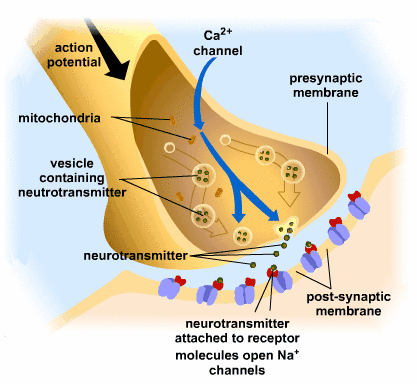
\includegraphics[width=.6\textwidth]{03_PlasticityInTheBrain/figures/synaptic_plasticity.jpg}
    \caption{Pre- and post-synaptic neuron}
    \label{fig:syn_plast}
\end{figure}


\paragraph{Synaptic Plasticity Alters the interneuron Connection Strength:} As the Amplitude of the EPSP increase it leads to a change in the producing and  receiving neuron. This allows the neuron to scale up or down in response to the received activity. In the short term the AMPA / NMDA channels increase, synaptic density size changes, in the long term (around 30 minutes) the number of spines increase thus creating more synapses 

\begin{figure}[H]
    \centering
    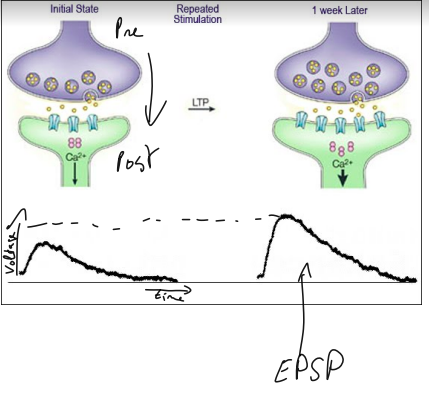
\includegraphics[width=.6\textwidth]{03_PlasticityInTheBrain/figures/pasted_image_1.png}
    \caption{}
    \label{fig:syn_plast1}
\end{figure}

\begin{figure}[H]
    \centering
    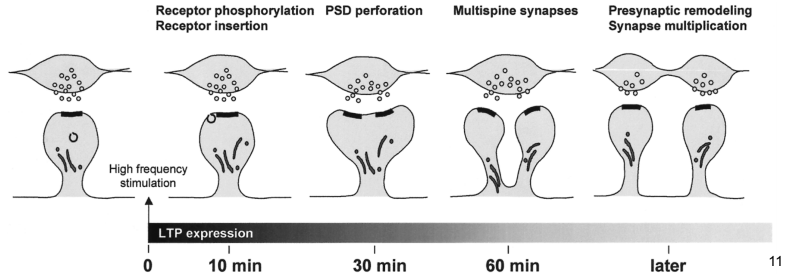
\includegraphics[width=.8\textwidth]{03_PlasticityInTheBrain/figures/pasted_image_2.png}
    \caption{}
    \label{fig:syn_plast1}
\end{figure}


\subsubsection{Homeostatic Plasticity}
\textit{Info in this section is extracted from the paper by Turrigiano \footnote{Turrigiano. Homeostatic Synaptic Plasticity: Local and Global Mechanisms for Stabilizing Neuronal Function. 2012.}.}\\

\noindent
Homeostatic plasticity is necessary to regulate neural circuits; to prevent them from becoming hyper- or hypo-active. In other words, homeostatic plasticity tries to break the positive feedback loop and make the neural circuit more stable. \\

\noindent But then, the question is \textbf{why would plasticity alone destabilize the activity of neural circuits?}
\begin{itemize}
    \item Although the synaptic-specific correlation-based mechanisms such as LTP and LTD contribute to learning and memory, they generate a powerful \textbf{destabilizing force} on network function. 
    \item This is because when synapses undergo LTP they are better able to depolarize the postsynaptic neurons, which will increase the probability that they will undergo further LTP—leading to \textbf{unconstrained synaptic strengthening}
    \item As correlated activity drives strengthening of specific synapses, and the post-synaptic neuron is driven more strongly, synapses that initially were only poorly correlated with postsynaptic firing will be better able to fire the postsynaptic neuron, so they too can be- come strengthened. Hence, the specificity breaks down.
\end{itemize}
For the above mentioned reasons, we therefore need forces to prevent further excitability and constraint the neural activity. To be considered truly homeostatic, a plasticity mechanism should regulate a key parameter (such as \textbf{average neuronal firing rate}) around some set-point value (See. fig.\ref{fig:firing_rate_regulation})

\paragraph{Example illustrating the importance of regulating the overall activity:}\footnote{Turrigiano and Nelson. Homeostatic Plasticity in the developing nervous system. \textit{Nature Reviews Neuroscience}.2004} One way to illustrate this is to consider the problem of propagating patterned activity from the sensory periphery to higher-order neurons deep within the brain. We can draw this as a feedforward hierarchical network as in fig. \cref{fig:feedforwardnet_instability} where the activity in each layer (for example, photorecep- tors, bipolar cells, ganglion cells, lateral geniculate neurons, primary visual cortical neurons, and so on) is driven by activity in the preceding layer. We can see that in this simplified topology, the gain of transmission from one layer to the next must be close to unity for propagation to occur, otherwise the signal either dies out or specificity is lost. This is because more neurons will be recruited at successive stages, and at the highest levels all neurons will fire regardless of the pattern of firing at the input layer.\\

\noindent
When information is propagated through a hierarchical network you want a certain amount of information expressed at each layer this prevent loss or explosion of information. This is similar to what occurs in deep networks, batch normalisation and weight decay, you want a certain activation so that there is not uniform de/activation in the layers.

\begin{figure}[H]
    \centering
    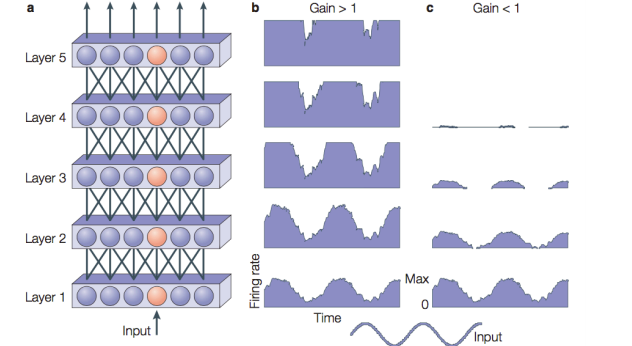
\includegraphics[width=.9\textwidth]{03_PlasticityInTheBrain/figures/pasted_image_5.png}
    \caption{The problem of stability in feedforward networks. a) Schematic feedforward network consisting of five layers of neurons. b,c) Expected firing rates of the red neuron in each layer in response to a sinusoidal input. If each action potential in a preceding layer causes more than one action potential in neurons at the next layer (b), the firing rates saturate and eventually all information about the stimulus is lost. If each action potential causes less than one action potential in neurons at the next layer (c), the signals eventually fail to propagate.}
    \label{fig:feedforwardnet_instability}
\end{figure}

\paragraph{Regulating the activity of a neuron around a set point:} There are many phenomema that contribute to stabilization of neuronal activity. An example is pre- and postsynaptic forms of excitatory synaptic plasticity, such as \textbf{synaptic scaling}, that adjust all of a neuron’s excitatory synapses up or down in the right direction to stabilize firing rate. Note that this scaling happens to all the synapses by the same "multiplicative" factor; therefore the relative synpatic stregth is preserved. 

\begin{figure}[H]
    \centering
    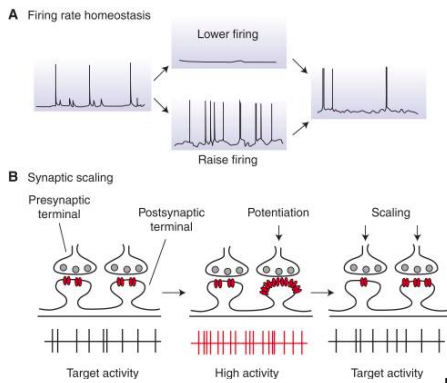
\includegraphics[width=.7\textwidth]{03_PlasticityInTheBrain/figures/pasted_image_4.png}
    \caption{Homeostasis of neuronal firing through homeostatic synaptic plasticity. (A) Cartoon illustration of the phenomenon of firing rate homeostasis in dissociated neocortical networks; perturbing firing in either direction results in the homeostatic regulation of synaptic and intrinsic properties so that baseline firing rates are restored. (B) One mechanism contributing to the firing rate homeostasis illustrated in A is synaptic scaling. When activity is perturbed (illustrated here as the potentiation of some inputs through Hebbian mechanisms) this triggers synaptic scaling, which \textbf{produces a proportional reduction in strength at all synapses} of the right magnitude to return firing to baseline levels. Note that, because this mechanism scales synaptic strength up or down proportionally, the relative difference in synaptic strengths induced by Hebbian mechanisms is preserved.[Caption extracted from paper].}
    \label{fig:firing_rate_regulation}
\end{figure}

\paragraph{Regulation of firing rate in cultured networks:} Initial observations using cortical cultures indicated that cortical pyramidal neurons maintain a set-point firing rate in the face of changing synaptic input. Cortical and other central neurons in culture form excitatory and inhibitory networks that develop spontaneous activity, and early studies found that blocking this activity for prolonged periods resulted in hyperactivity in these networks when activity was allowed to resume. The reciprocal manipulation — elevating network activity by reducing a fraction of inhibition — initially raises firing rates, but over many hours firing rates fall again until they approach control levels.

\begin{figure}[H]
    \centering
    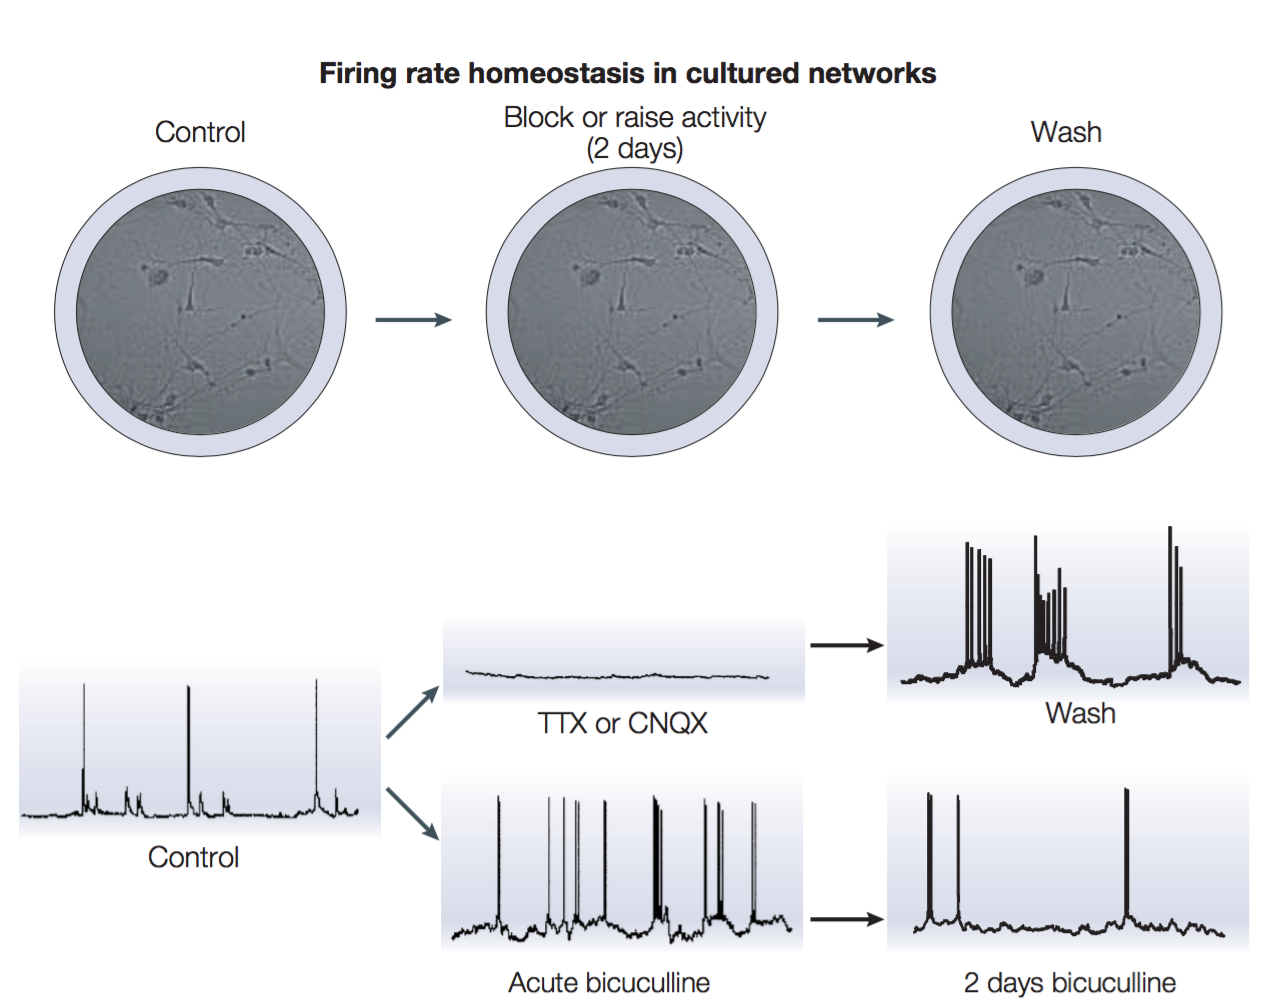
\includegraphics[width=.9\textwidth]{03_PlasticityInTheBrain/figures/firing_rate_homestatis.png}
    \caption{Evidence for firing rate homeostasis in cultured networks. Cultured cortical networks are composed of interconnected excitatory pyramidal and inhibitory interneurons, and develop spontaneous activity after a few days in vitro (control). This activity can be pharmacologically manipulated for long periods. Blockade for two days of spiking activity with tetrodotoxin (TTX), or of excitatory glutamagergic synapses with CNQX, generates a rebound phenomenon whereby the excitability of the network is increased when the drugs are removed (wash). A more direct test of the idea of firing rate homeostasis is to raise activity acutely with bicuculline (acute bicuculline), and then to follow activity over time. After two days in bicuculline, activity has returned almost to control levels (2 days bicuculline). These experiments, and others like them, indicate that homeostatic mechanisms adjust the cellular and synaptic properties of cortical networks to compensate for changes in synaptic drive.}
    \label{fig:homeostatis_cultured_nets}
\end{figure}


% Example: isolated neurons are given inhibitors or excitatory chemical. Then washed the chemical effects off and the neuronal activity will spike in the inhibitory neurons and decrease in the artificially excited neurons. 



\subsubsection{Hebbian Plasticity}
There are two major forms of plasticity in thenervous system: Hebbian plasticity and homeostatic plasticity.  Hebian plasticity can be considered as a special form of homestatic plasticity. \\

\noindent
Hebbian plasticity is a synaptic-basis for associative learning. In this form of plasticity synapses change their number in relation to the stimulated synapses. So, it is \textbf{synaptic-specific}. On the other hand, in homestoatic plasticity, as mentioned in the previous section, the synaptic scaling affects all the synapses (more global change in order to maintain the activity of the neural circuit around a target point).

\begin{figure}[H]
    \centering
    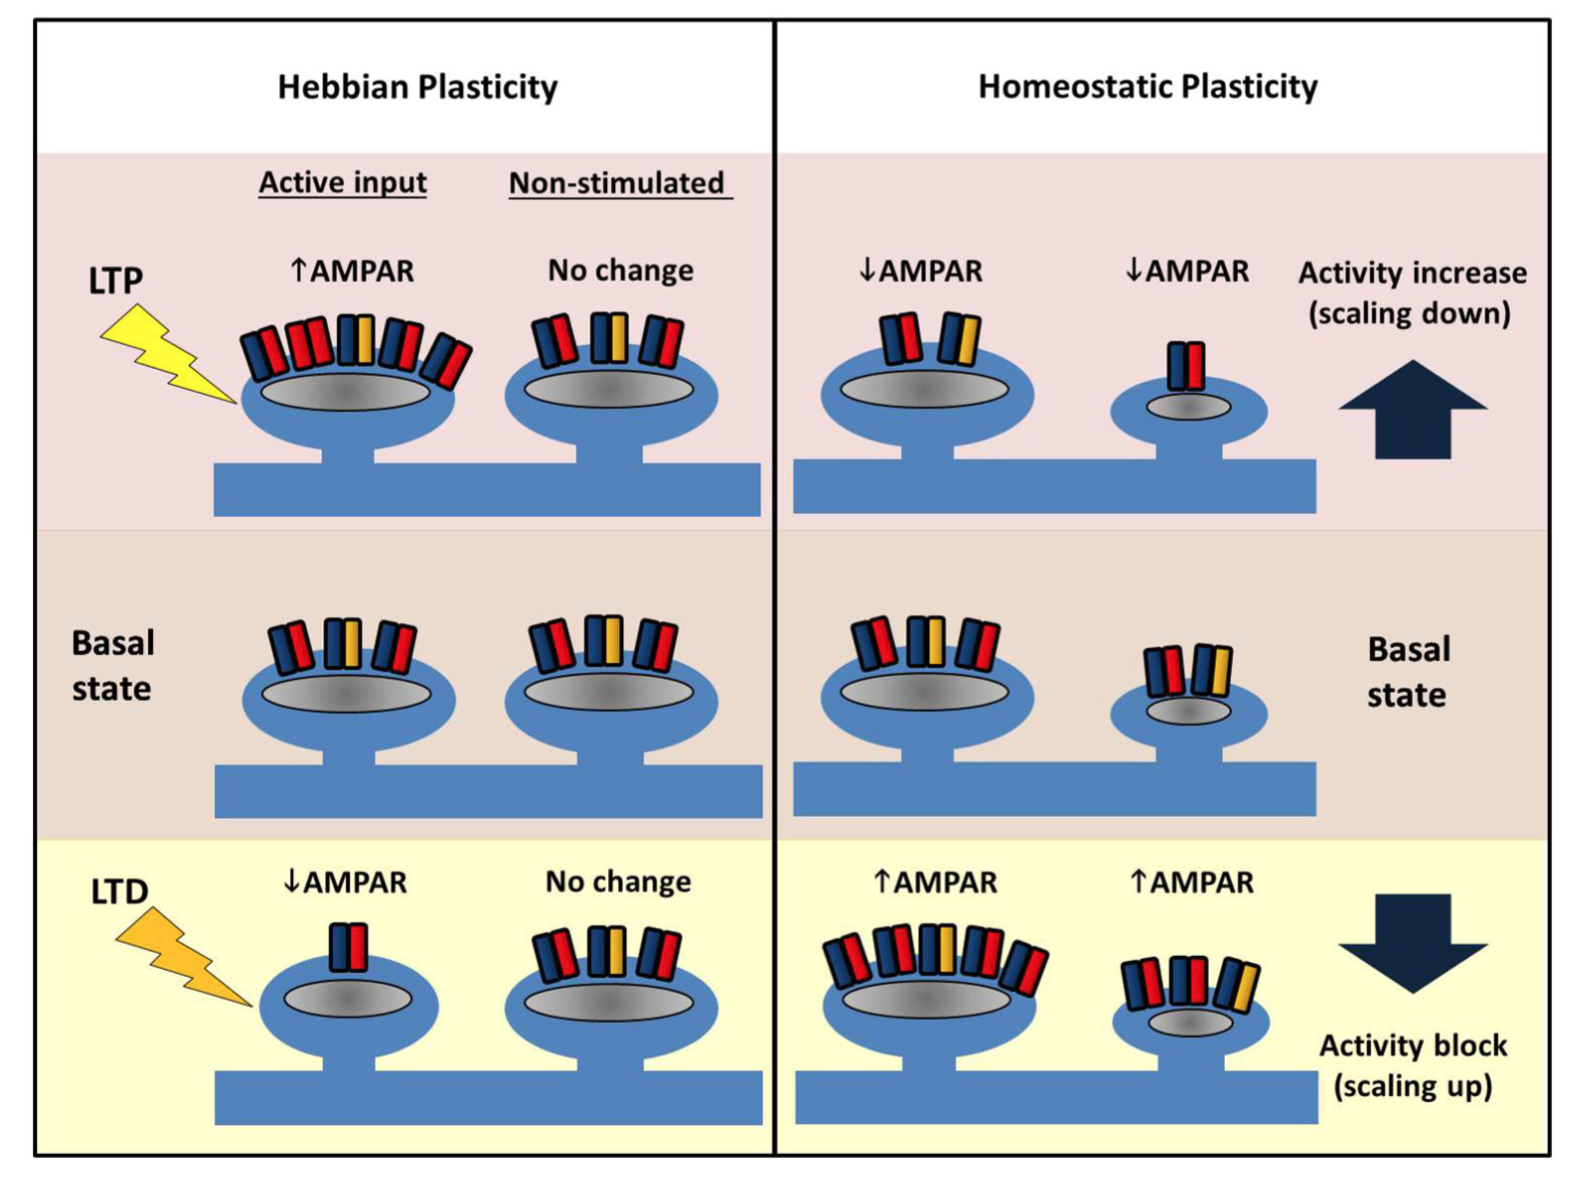
\includegraphics[width=.9\textwidth]{03_PlasticityInTheBrain/figures/hebbian_vs_homeostatic.png}
    \caption{Comparing Hebbian and homeostatic plasticity. During Hebbian forms of plasticity synapses change their number of AMPARs in an input-specific fashion. Different patterns of activity can either cause strengthening (LTP, top left) or weakening of synapses (LTD, bottom left) via AMPAR trafficking. Potentiation or depression is limited to stimulated synapses, and neighbors are unaffected. In contrast, during homeostatic plasticity altered levels of neuronal activity drives changes in synaptic AMPAR number across the entire dendritic arbor. Blocking pre- and postsynaptic spiking with TTX causes AMPARs to accumulate at excitatory synapses (bottom right). Conversely increasing network activity (for example with a $GABA_A$R antagonist) causes a reduction in synaptic AMPAR (top right). Crucially this form of plasticity conserves the relative strength difference between synapses.}
    \label{fig:hebbian_vs_homeostatic}
\end{figure}




\subsubsection{Some biological notions}
\begin{itemize}
    \item Synaptic scaling = Scaling up or down of the quantal amplitude of all synapses onto a postsynaptic neuron in response to long- lasting changes in neuronal activity.
    \item Hebbian plasticity = changes in the connection strength between two neurons as a result of correlated firing.
    \item AMPARS = a subtype of ligand-gated glutamate receptor; these receptors generate the majority of excitatory current at central synapses.
\end{itemize}


% -----------------------------
\newpage
\subsection{Hebbian Learning}

\paragraph{Hebb's synapse:} As described by Donald Hebb in \textit{The Organization of Behavior}(1949), “When an axon of cell A is near enough to excite cell B and \underline{repeatedly} or \underline{persistently} takes part in firing it, some growth process or metabolic change takes place in one or both cells such that A's efficiency, as one of the cells firing B, is increased.”.  Hebb postulated that this behavior of synapses in neuronal networks would permit the networks \textbf{to store memories}.\\

\noindent
We can consider that a \textbf{Hebbian synapse is a “coincidence detector”}.

\begin{figure}[H]
    \centering
    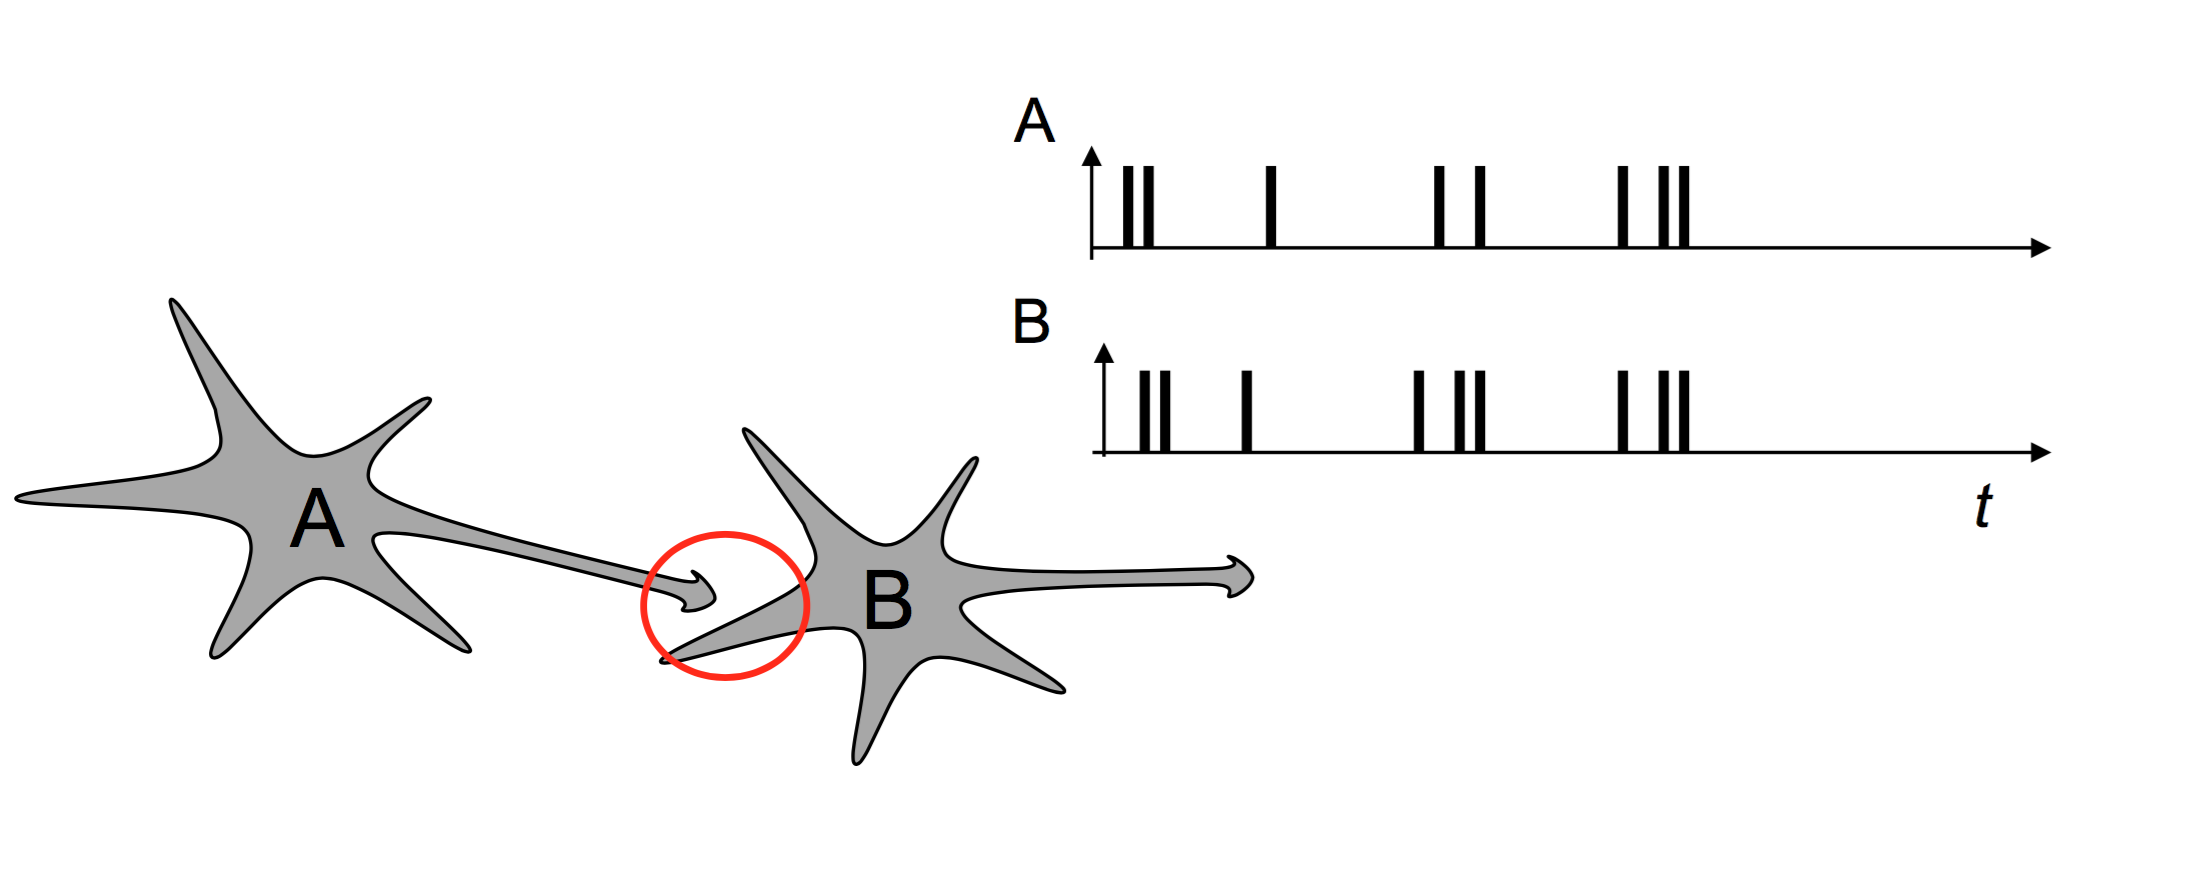
\includegraphics[width=.9\textwidth]{03_PlasticityInTheBrain/figures/Hebb_synapse.png}
    \caption{Hebb's synapse.}
    \label{fig:hebb_synapse}
\end{figure}

\noindent

\paragraph{Recap}
\begin{itemize}
    \item Tuning of synapses as seen in homeostatic plasticity can be seen at specific individual synapses. When this occurs it is known as hebbian plasticity. The synapses strength increases to specifically activated neurons. Those neurons that fire together wire together associativity.  
    \item There also can be cooperativity whereby multiple cells are required for spiking. This brings in the idea of associative learning whereby multiple features of an object linked together as it allows for better firing. 
\end{itemize}

\subsubsection{Spike-Timing Dependent Plasticity (STDP)}
\begin{itemize}
    \item STDP is a \textbf{temporally asymmetric} form of Hebbian learning induced by tight temporal correlations between the spikes of pre- and postsynaptic neurons\footnote{\url{http://www.scholarpedia.org/article/Spike-timing_dependent_plasticity}}.
    \item It is observed that repeated pre-synaptic spike arrival a few milliseconds before postsynaptic action potentials leads in many synapse types to Long-Term Potentiation (LTP) of the synapses. Therefore, the synaptic weight is increased.
    \item On the other hand, repeated spike arrival after postsynaptic spikes leads to Long-Term Depression (LTD) of the same synapse, where the synaptic weight is reduced.
\end{itemize}

\begin{figure}[H]
    \centering
    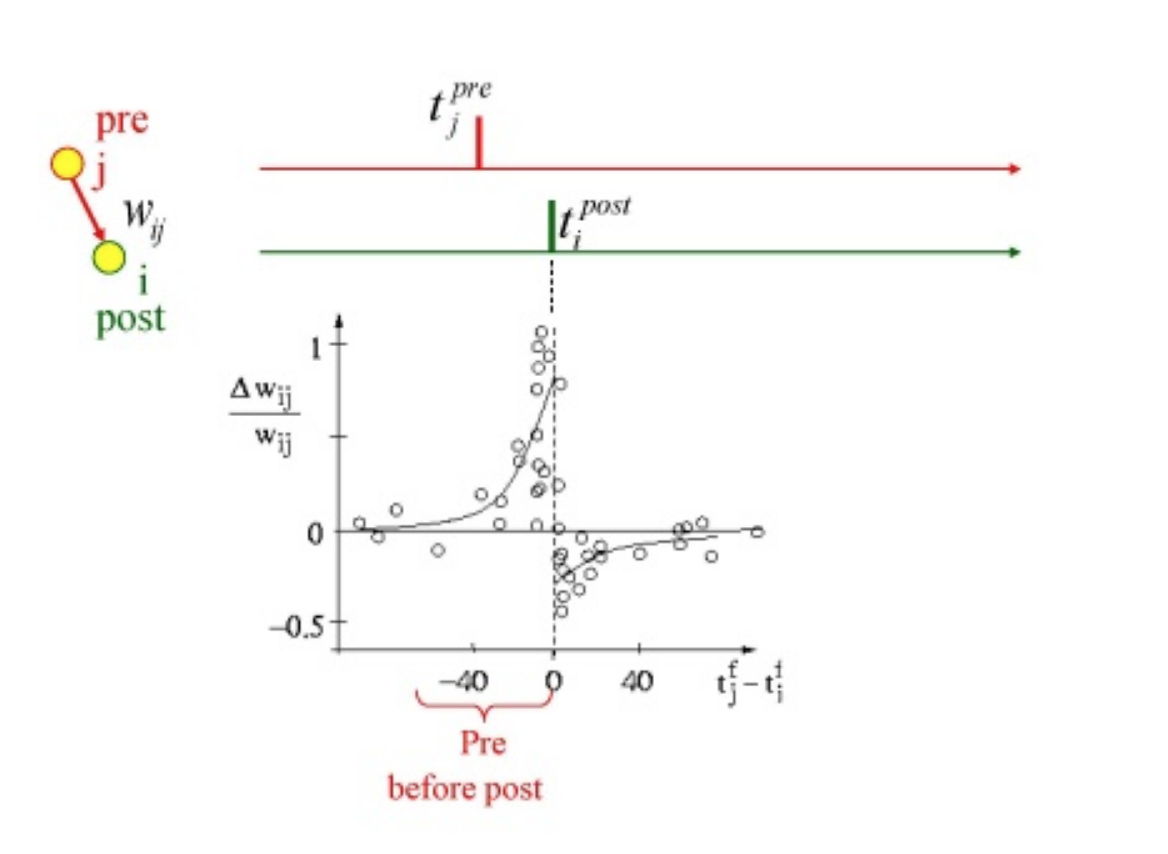
\includegraphics[width=.9\textwidth]{03_PlasticityInTheBrain/figures/STDP.png}
    \caption{Spike-Timing Dependent Plasticity (schematic): The STDP function shows the change of synaptic connections as a function of the relative timing of pre- and postsynaptic spikes after 60 spike pairings. Schematically redrawn after Bi and Poo (1998) (Note that the y-axis is normalized).}
    \label{fig:STDP}
\end{figure}



\begin{figure}[H]
    \centering
    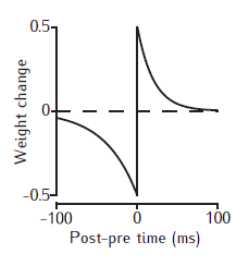
\includegraphics[width=.5\textwidth]{03_PlasticityInTheBrain/figures/pasted_image_6.png}
    \caption{STPD, spike timing dependent activity, graph if the post is active then per gave input no weight change (LTD) should occur. If the post fired then activated the pre then weight increased (LTP) should occur.}
    \label{fig:syn_plas1t}
\end{figure}

\begin{equation}
\begin{array}{l}
{\dot{w}=H(\text { pre, post })} \\
{\dot{w}=F(M, \text { pre, post })}
\end{array}
\end{equation}
    

Writing down hebbian learning it can be thought of as a H a function that detects the correlation of pre and postsynaptic potentials leading to a weight change. 



\subsubsection{Hebb's idea and associative memory: Hebbian cell assembly}
\begin{itemize}
    \item Synaptic plasticity helps us form memories that we can recall at a later stages in our lives.
    \item One of the most iconic concepts of memory formation is the notion of the \textbf{Hebbian cell assembly}. Under this notion, \textbf{Hebbian learning is believed form associative memory traces or engrams}.
    
\end{itemize}
\paragraph{Hebbian cell assembly:} "A Hebbian cell assembly is formed when an ensemble of neurons is repeatedly co-activated. This co-activation is thought to trigger experience-dependent “Hebbian plasticity” which causes a strengthening of the excitation connections between the co-active neurons. This so formed assembly can now be seen as an associative memory engram. The memory can be recalled by only activating a subset of the neurons within a given assembly. By dint of the strong connections, the activity can then spread to re-activate the whole assembly."\footnote{https://zenkelab.org/research/synaptic-plasticity-and-homeostasis/}

\begin{figure}[H]
    \centering
    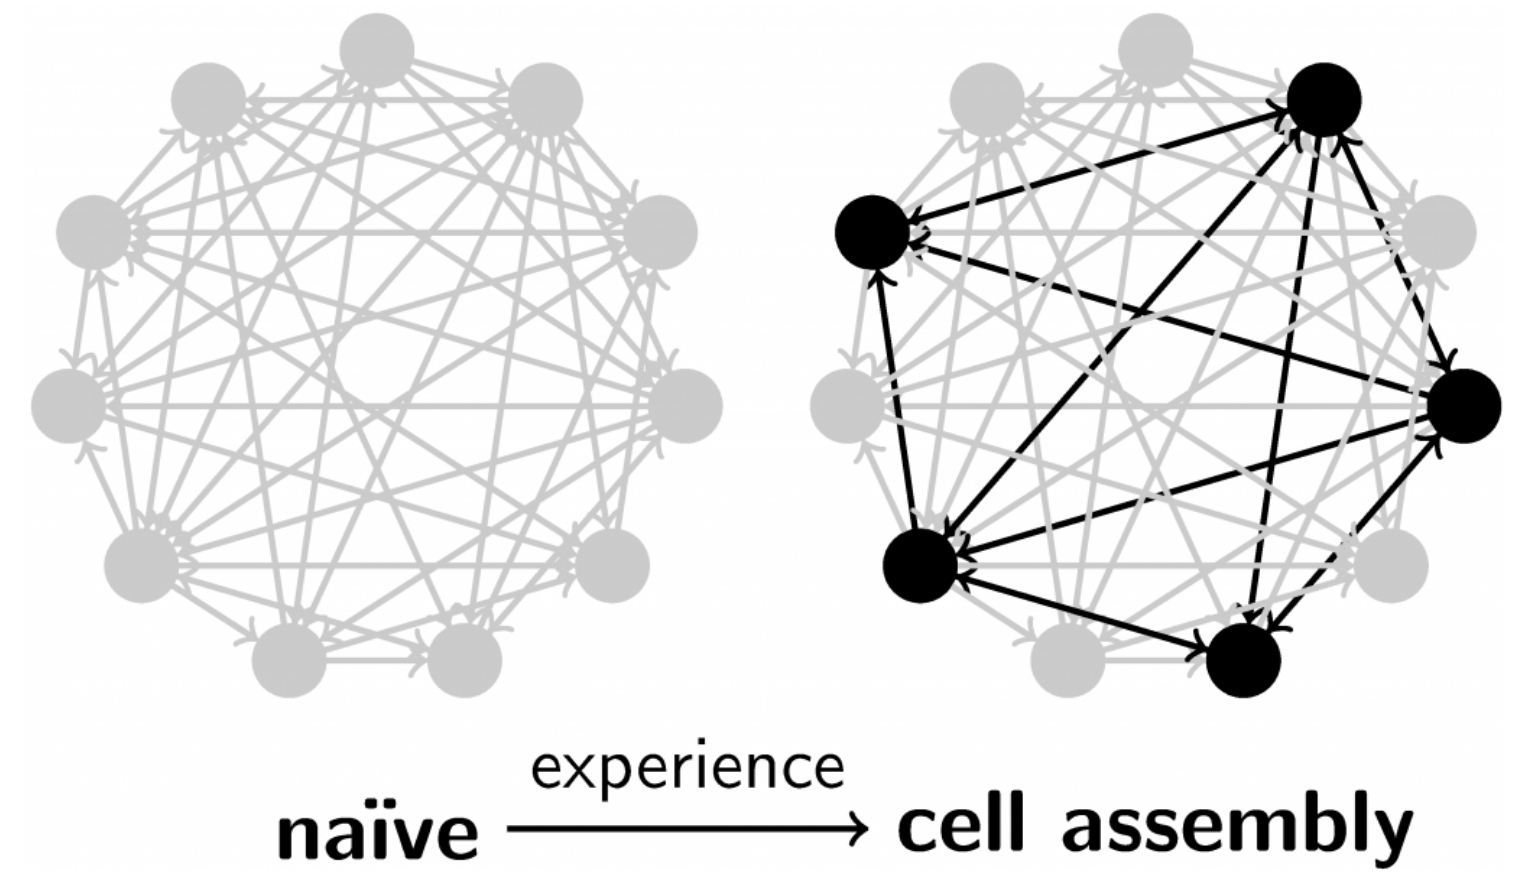
\includegraphics[width=.8\textwidth]{03_PlasticityInTheBrain/figures/hebb_cell_assembly.png}
    \caption{Formation of Hebbian cell assembly with experience}
    \label{fig:cell_assembly}
\end{figure}

\paragraph{Specificity and associativity:} Both are consequences of Hebbian rule.
\begin{itemize}
    \item \textbf{Specificity} implies that only pre-synaptic neurons that are active during the depolarization of the post-synaptic neuron tend to have their synapse on the post-synaptic neuron strengthened.
    \item \textbf{Associativity} implies that two pre-synaptic neurons who fire at the same time, together depolarizing the same post-synaptic cell, will tend to have their synapses on the post-synaptic cell strengthened \textbf{MORE} than if either of the two cells had fired individually--the greater degree of depolarization due to the cells firing together causes the two pre-synaptic neurons to associate on the post-synaptic neuron. Further, pre-synaptic cells that have a strong synapse on a post-synaptic cell can have the effect of pulling other more weakly connected cells towards the post-synaptic cell if the other cells fire at the same time as the stronger-synapsing cell.
\end{itemize}
\begin{figure}[H]
    \centering
    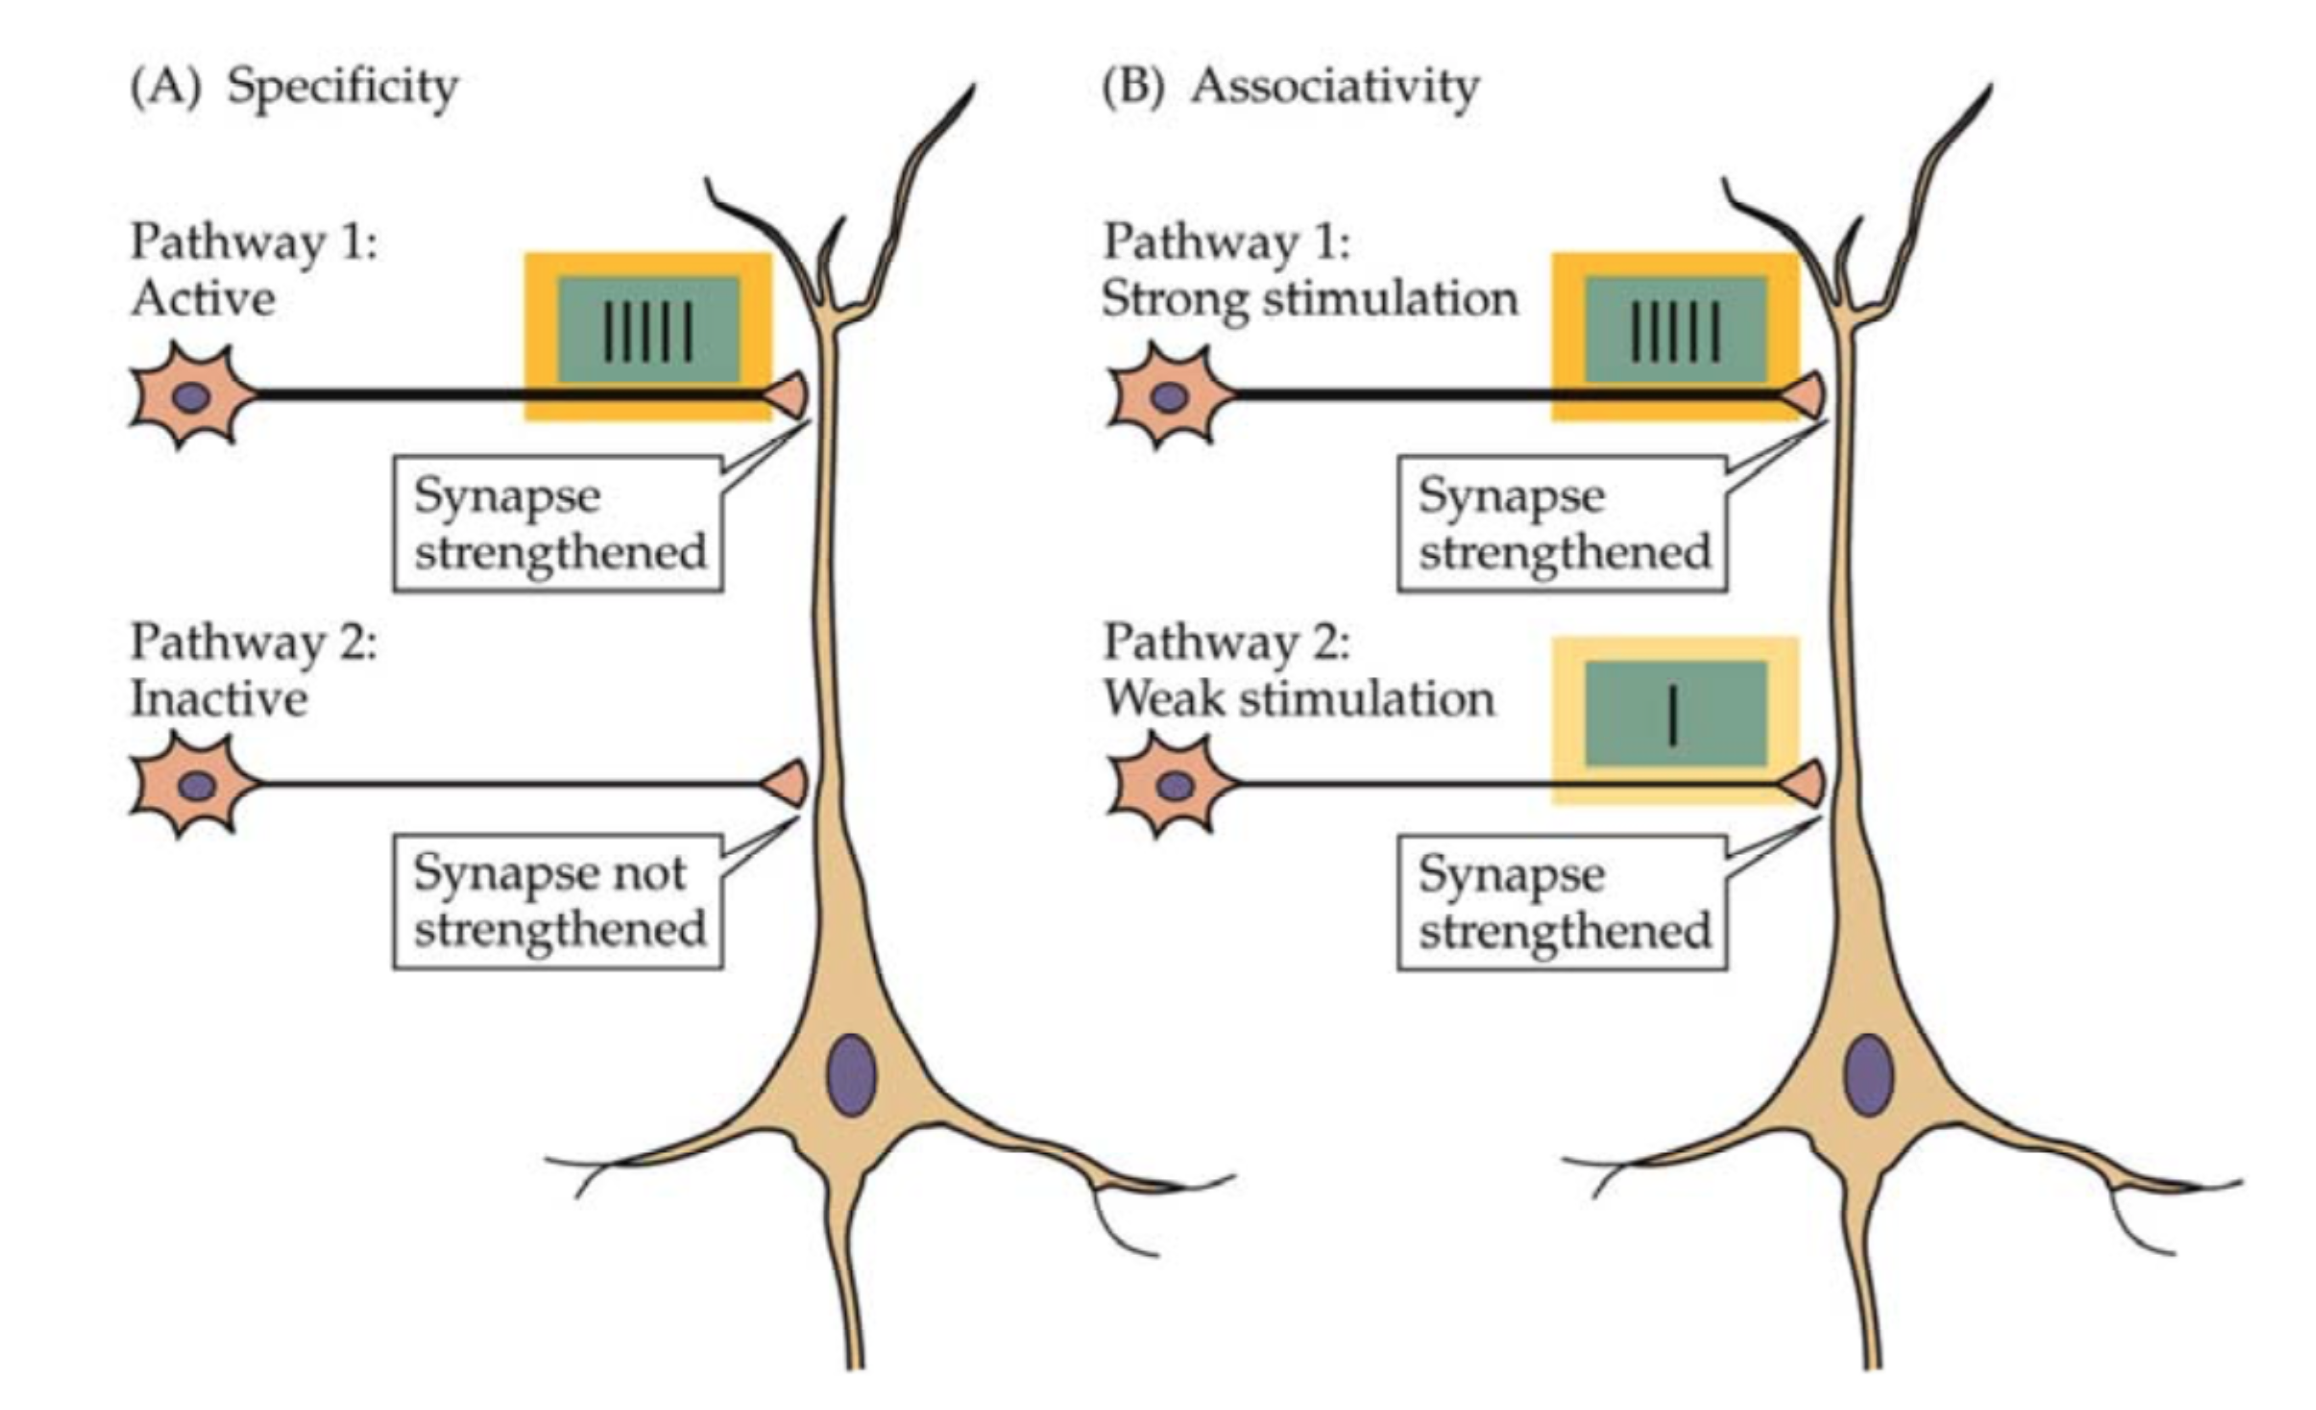
\includegraphics[width=.8\textwidth]{03_PlasticityInTheBrain/figures/specificity_associativity.png}
    \caption{Two consequences of Hebbian rule: specificity and associativity}
    \label{fig:specificity_associativity}
\end{figure}


\subsubsection{The Problem with Hebbian Learning}
One of the main concerns of Geoffrey Hinton regarding Hebbian learning is that lack of a teaching signal. In other words, this learning rule is not error-driven; synaptic weights are updated relying on the correlation between the pre- and post synaptic activities. In his paper \footnote{The Ups and Downs of Hebb Synapses. 2003}, he states that even for rather simple tasks, the "Hebbian" approach was seen as "inferior" to other error-driven methods that use the product of the pre-synaptic activity and the post-synaptic activity derivatives.\\

\noindent
In backprop, the neurons are trained so that everyone is optimised. These errors are important for hierarchical learning to gain correct responses. \\

\noindent
One solution for this problem is\textbf{ three-factor Hebbian learning.} 
\subsubsection{Three-Factor Hebbian Learning}
Associative (Hebbian) learning indicates association between \textbf{two factors} (two sensory inputs or an input and an output). Here the idea is to introduce another factor for modulating the plasticity. This additional factor "may represent, for example, rewards, supervised errors, summary statistics, or attentional feedback, which could be used to facilitate different types of learning by providing more global information about how well the whole network is performing or how important a current situation is."\footnote{Kusmierz,Isomura and Toyoizumi. Learning with three factors: modulating Hebbian plasticity with errors. Current Opinion in Neurobiology.2017}. \\

This rule can hence be written as follows:
\begin{equation}
    \dot{w}= F(M,\; pre, \;post)
\end{equation}

Three-factor rules have also been called “neoHebbian” (Lisman et al., 2011; Lisman, 2017) or \textbf{"heterosynaptic" (modulatory-input dependent)}.

The M acts as the third factor, it could be the error that allows it to become error driven. Biologists are examining this could be a global reward like dopamine or local activity. 

% --------------------------------------
\subsection{Non-Hebbian Plasticity: Heterostatic Plasticity}
There are two broad categories of synaptic plasticity, generally referred to as \textbf{homosynaptic} and \textbf{heterosynaptic} plasticity.

\begin{itemize}
    \item Homostatic plasticity is what we have been discussing with the Hebbian syapases: a synapse-specific strengthening (facilitation) or weakening (depression) based on the activity of pre- and post-synaptic neurons. In fact the three characteristics: homosynaptic plasticity, associativity and input specificity form the modern definition of the Hebbian synapse.
    
    \item Heterostatic plasticity refers to synaptic weight adaptation (facilitation or depression) based on the firing of a third modulatory interneuron. It is therefore referred to as non-hebbian plasticity.
    
\end{itemize}


\begin{figure}[H]
    \centering
    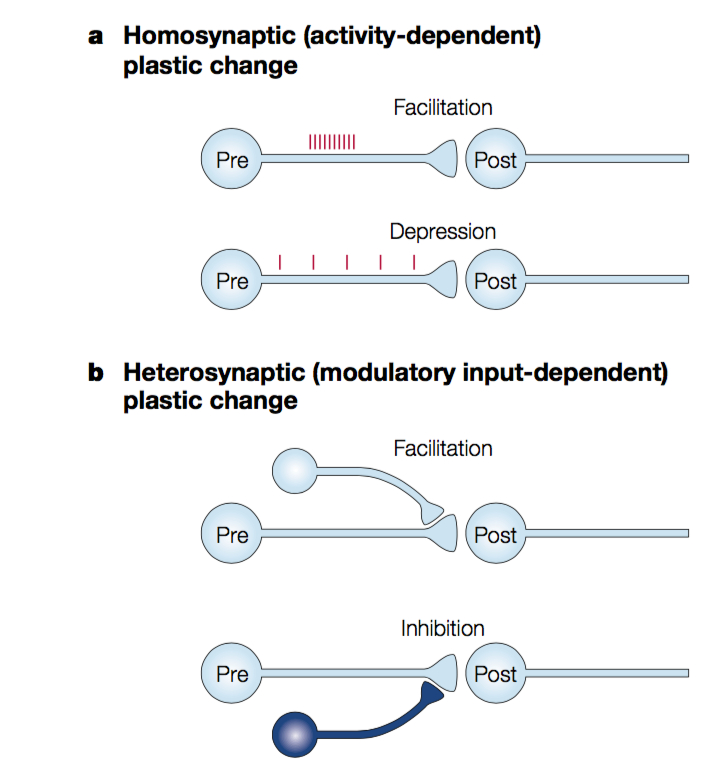
\includegraphics[width=.8\textwidth]{03_PlasticityInTheBrain/figures/homostatic_heterostatic.png}
    \caption{Homosynaptic and heterosynaptic mechanisms for long-term plasticity. a) The plastic changes that underlie long-term memory follow a homosynaptic rule, that is, the events responsible for triggering synaptic strengthening occur at the same synapse as is being strengthened. These changes can result in an increase in synaptic strength (for example, homosynaptic facilitation), or a decrease in synaptic strength (for example, homosynaptic depression). b) Synaptic strengthening between a presynaptic and a postsynaptic cell can occur as a result of the firing of a third neuron, a modulatory interneuron, whose terminals end on and regulate the strength of the specific synapse. These changes can result in an increase (heterosynaptic, modulatory facilitation) or in a decrease (heterosynaptic inhibition) in synaptic strength}
    \label{fig:syn_plas1t}
\end{figure}

Is the modulation of the input into the post from the presynaptic neuron. This then leads to the change in the post either facilitatory with excitatory inputs or inhibitory with inhibitory inputs. 

Example Fly: neurons come into a brain area these act to modulate postsynaptic neurons. With greater activation the pre synatpic neurons grow irrespective of the postsynaptic activity.

Example 2: A the brain receives a reward it acts to modulate the synapse. It then changes the STDP profile it causes an increase in the synaptic strength irreseptic if the post or pre fires first. This is known as a Heterostatic Modulation.


\subsubsection{Behavior time scale Plasticity}




\subsubsection{Time scales of synaptic plasticity (short term, LTP/LTD)}
STP and STD (short term depression and potentiation) this occurs in the short term memory seconds to minutes, LTD and LTP occurs between seconds to minutes. 
The longer time scales the formation of new synapses as result short term processes hours to months. 
Then the ultra long time scales is the structural changes in brain regions. Months to lifetime.

This can be summarized as:
\begin{enumerate}
    \item Short term facilitation/depression [seconds to hours]
    \item Long term facilitation/depression
    \item Generation of new synapses (synaptic pruning) [hours to months]
    \item Structural changes in neuronal networks [months to lifetime]
\end{enumerate}



\begin{figure}[H]
    \centering
    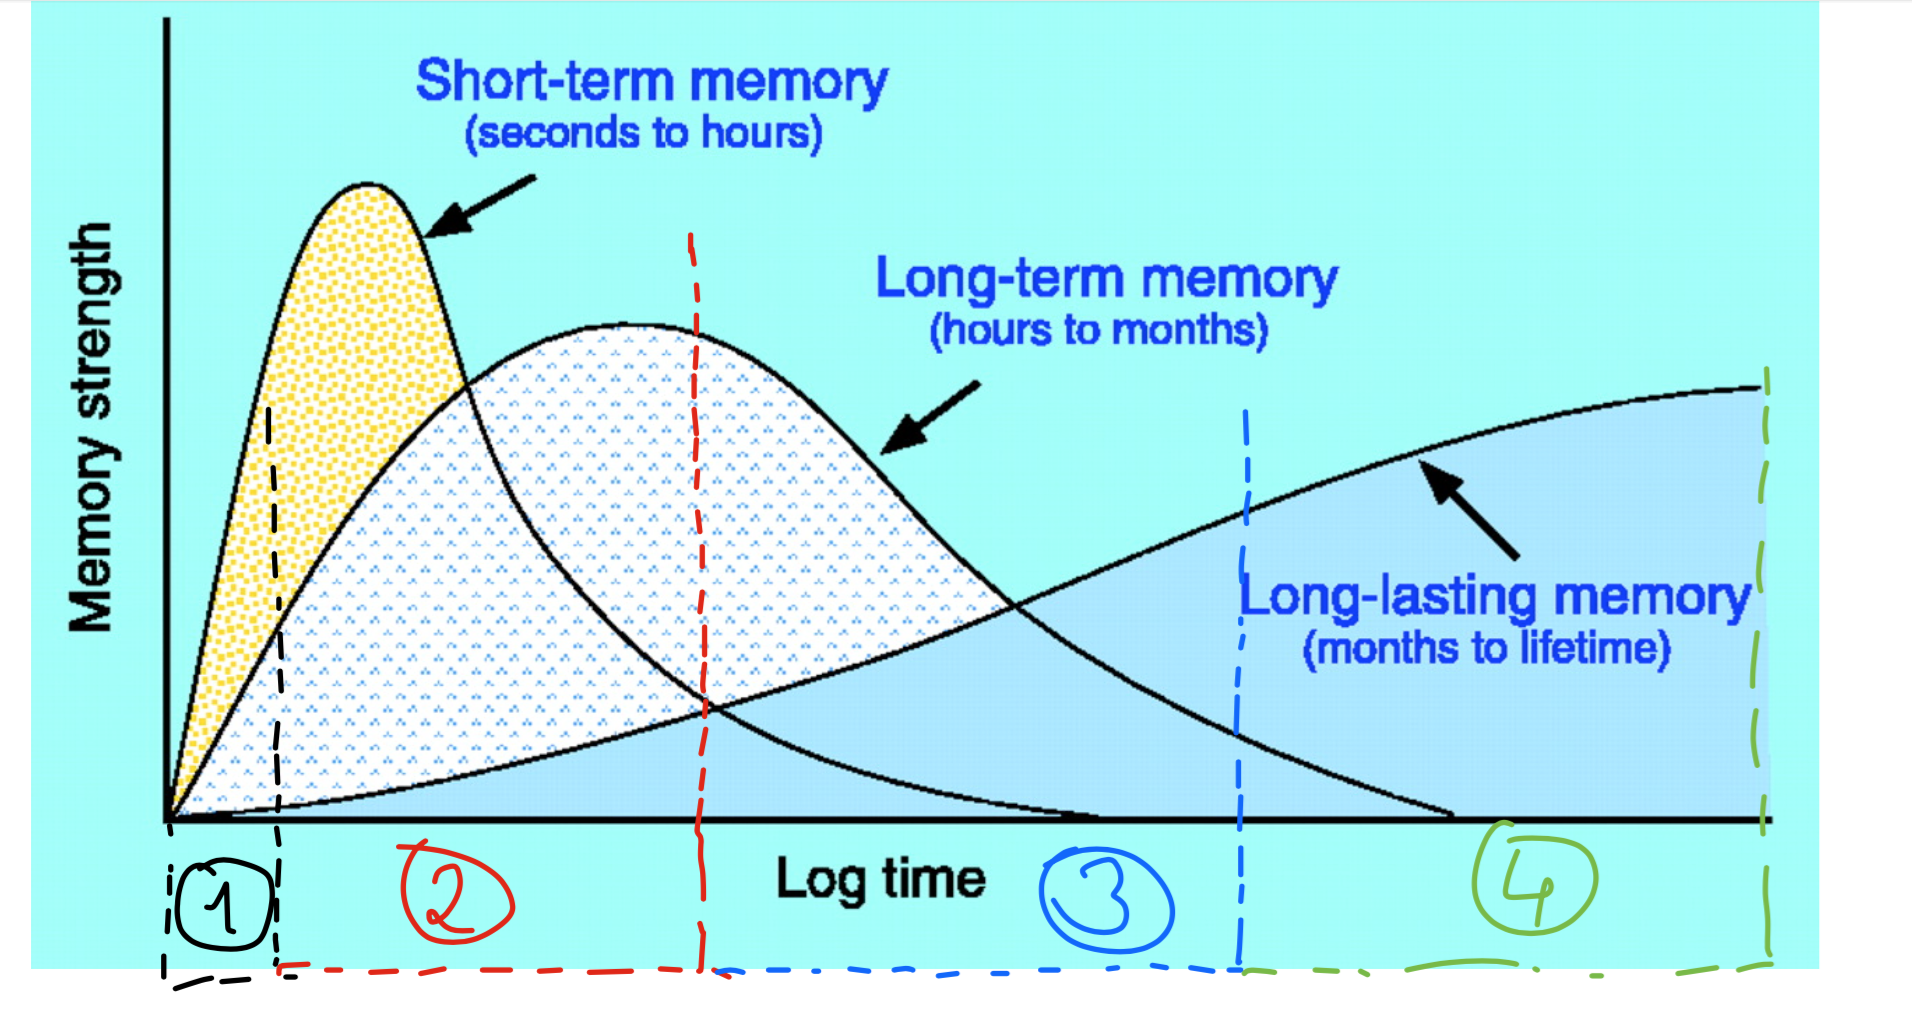
\includegraphics[width=.8\textwidth]{03_PlasticityInTheBrain/figures/timescale_plasticity.png}
    \caption{Timescales of Neuronal Plasticity}
    \label{fig:timescales}
\end{figure}

\subsubsection{Short term plasticity (STP)}
Once again, there are two types of short-term plasticity (STD): Short-Term Depression (STD) and Short-Term Facilitation (STF). 

\begin{itemize}
    \item [--]STD is caused by depletion of neurotransmitters consumed during the synaptic signaling process at the axon terminal of a pre-synaptic neuron, 
    \item [--] STF is caused by influx of calcium into the axon terminal after spike generation, which increases the release probability of neurotransmitters
    \item [--]STP has been found in various cortical regions and exhibits great diversity in properties (Markram et al., 1998, Dittman 2000, Wang 2006)).
    \item [--]Synapses in different cortical areas can have varied forms of plasticity, being either STD-dominated, STF-dominated, or showing a mixture of both forms.
\end{itemize}

\begin{figure}[H]
    \centering
    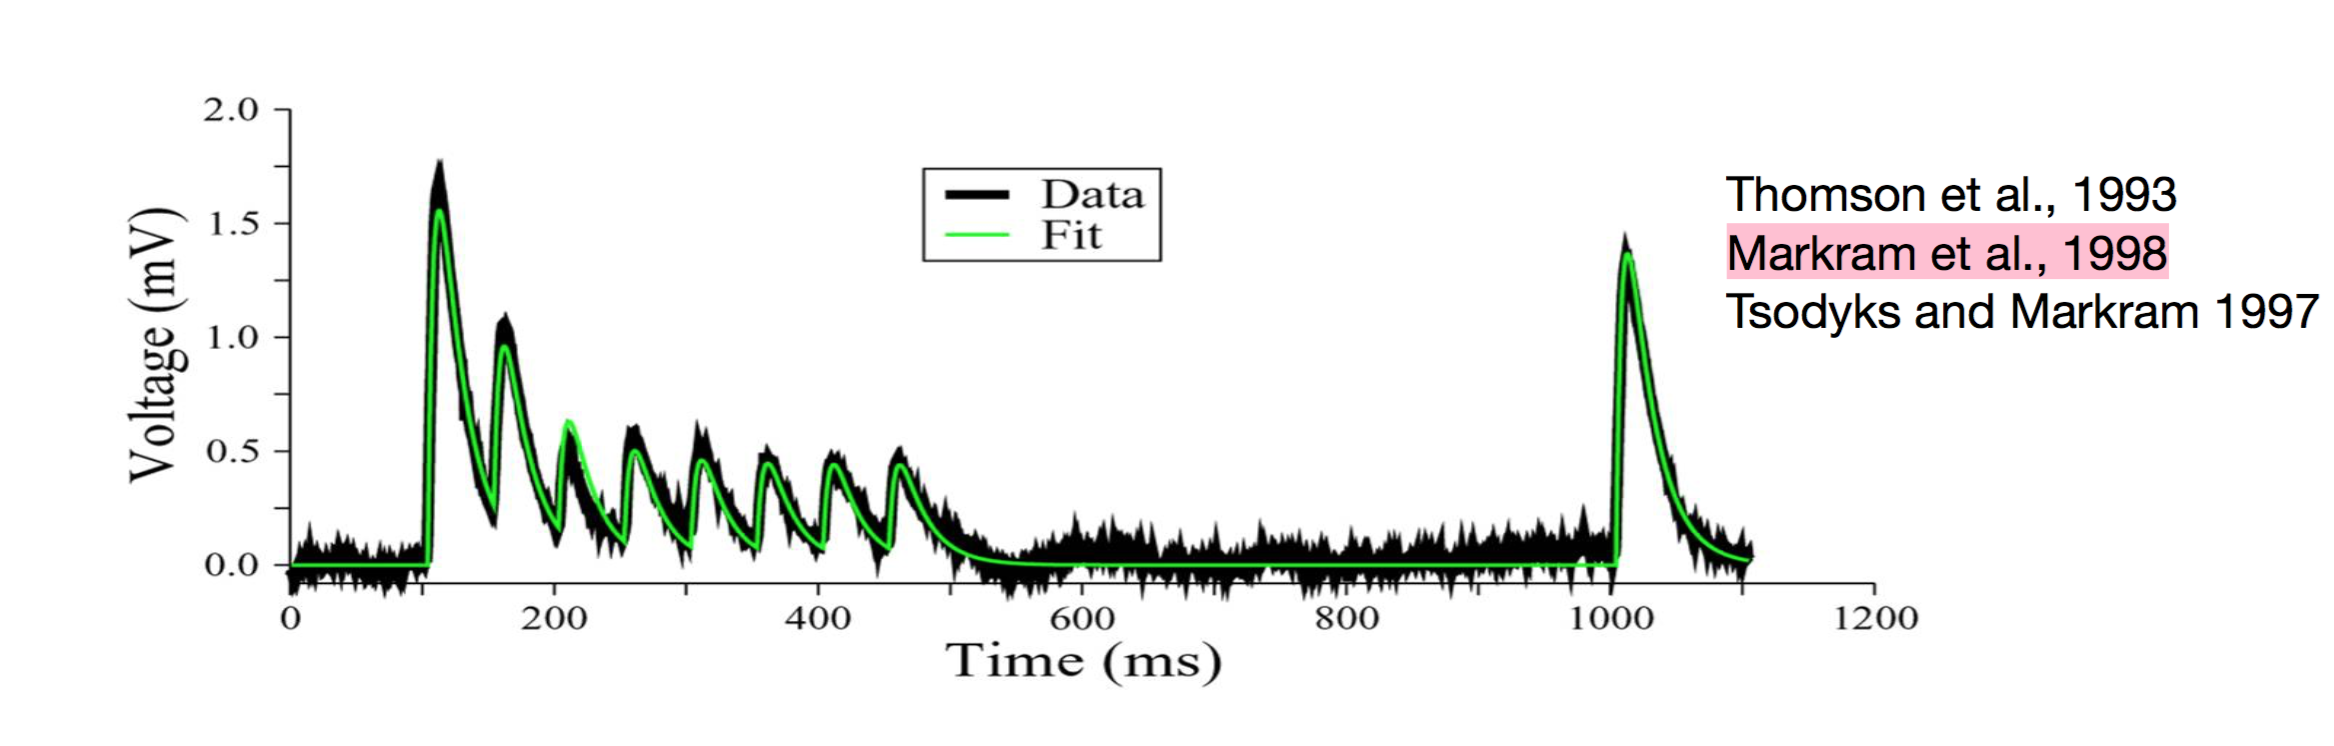
\includegraphics[width=.8\textwidth]{03_PlasticityInTheBrain/figures/STD.png}
    \caption{Short-term depression}
    \label{fig:STD}
\end{figure}

%---------------------------
\subsection{The Hippocampus as a model system to study neural plasticity}
Hippocampus (HC) is a model system of learning and memory. \\
\noindent
Role of HC in learning and memory has been shown with rat experiments with the Morris Water Maze(MWM). MWM is large pool of opaque water where the rats are placed. The rats were trained to find and escape onto a platform which was hidden. Authors show that chronic infusion of an NMDA antagonist leads to impairment in place learning.\\

\noindent
\underline{\textbf{To summarize:}}
\begin{itemize}
    \item Recent work has shown that the hippocampus contains a class of receptors for the excitatory amino acid glutamate that are activated by N-methyl-D-aspartate (NMDA) and that exhibit a peculiar dependency on membrane voltage in becoming active only on depolarization.
    \item Blockade of these sites with the drug aminophos-phonovaleric acid (AP5) does not affect synaptic transmission in the hippocampus, but \textbf{prevents the  LTP} following brief high- frequency stimulation.

\end{itemize}

% is tracked with a camera. Over time the mouse will learn where the platform is. If certain receptors important to LTP and LTD  are blocked, the mouse does not learn. It shows that the learning is dependant on synaptic plasticity and hippocampus.

\subsubsection{Most studied synapse in HC: CA3 $\rightarrow$ CA1}
\begin{itemize}
    \item The main pyramidal cell layers in HC are the CA1-4 regions (principally CA1 and CA3) and the dentate gyrus.

\end{itemize}

 \paragraph{Schaffer Collateral/Associational Commissural Pathway:}\footnote{\url{http://www.bristol.ac.uk/synaptic/pathways/}} This pathway is derived from axons that project from the CA3 region of then hippocampus to the CA1 region. The axons either come from neurons in the same hippocampus (ipsilateral) or from the other hippocampus (contralateral). These latter fibres are termed commissural fibres, as they cross from one hemisphere of the brain to the other. This pathway is utilised very extensively exhibits to study NMDA receptor-dependent LTP and LTD.
 
 \begin{figure}[H]
    \centering
    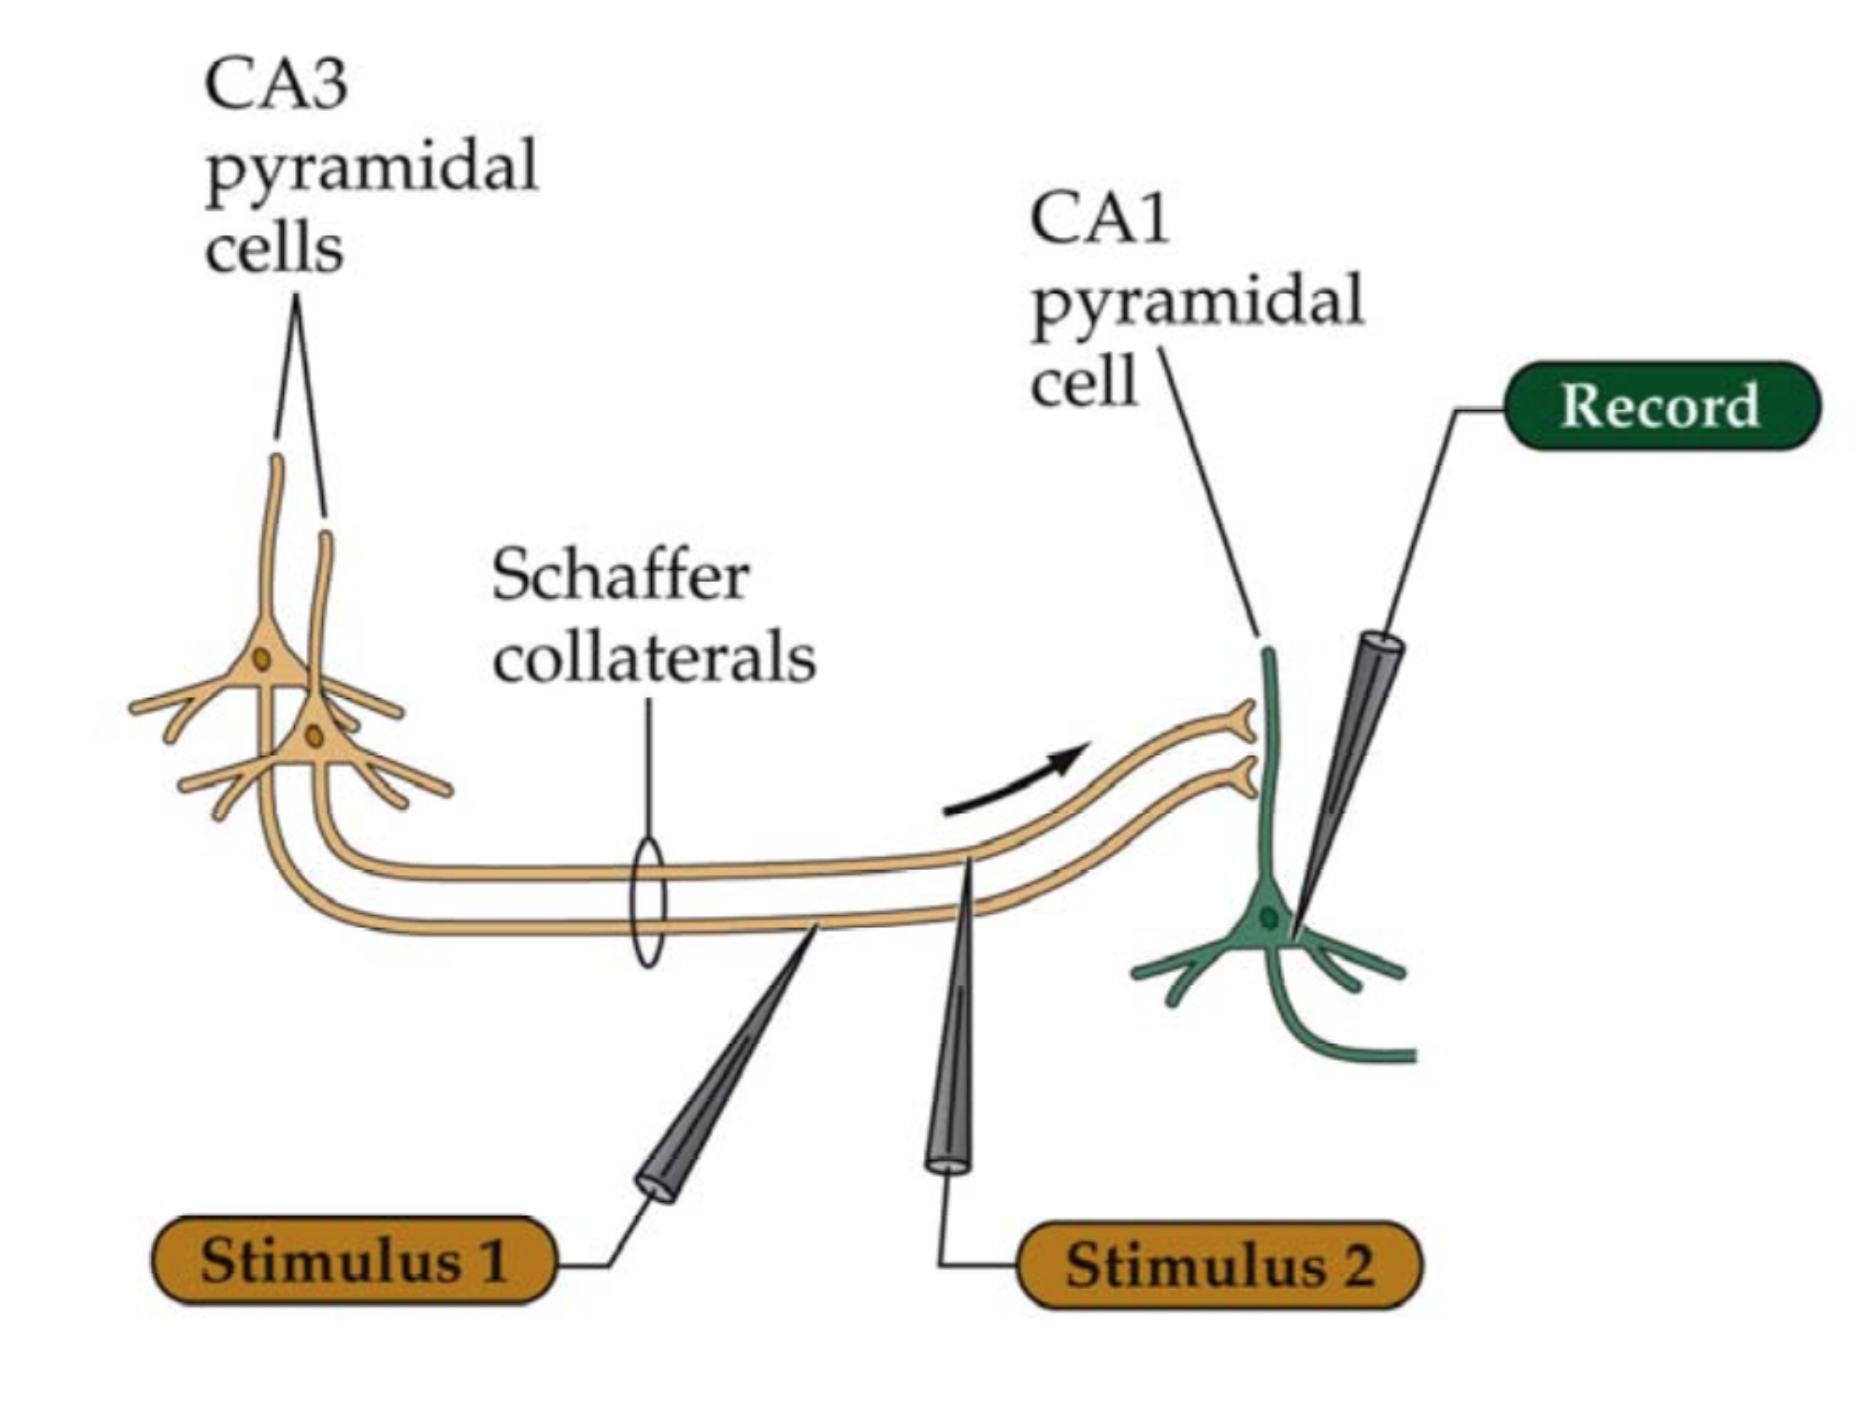
\includegraphics[width=.6\textwidth]{03_PlasticityInTheBrain/figures/ca3_ca1.png}
    \label{fig:HC_synapses}
\end{figure}
    


\begin{figure}[H]
    \centering
    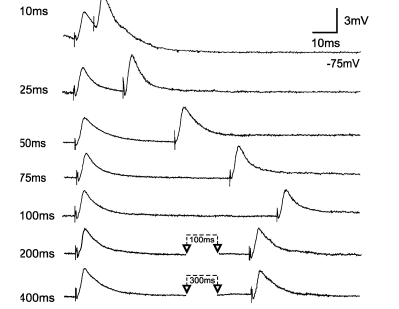
\includegraphics[width=.6\textwidth]{03_PlasticityInTheBrain/figures/pasted_image_9.png}
    \caption{Heterostatic Plasticity}
    \label{fig:syn_plas1t}
\end{figure}

\begin{figure}[H]
    \centering
    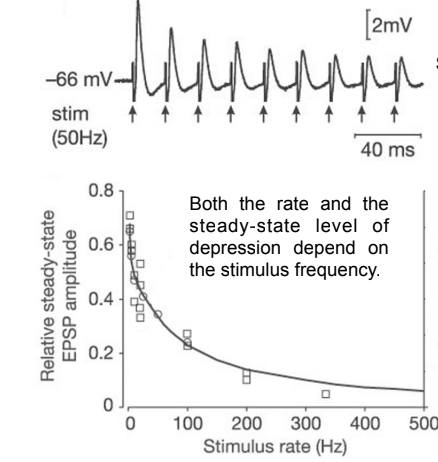
\includegraphics[width=.6\textwidth]{03_PlasticityInTheBrain/figures/pasted_image_10.png}
    \caption{Heterostatic Plasticity}
    \label{fig:syn_plas1t}
\end{figure}

To test plasticity in the hippocampus the Ca3 to Ca1 pathway was modulated and the EPSP in the Ca1 was measured, this tells you the activity of the pathway. If the spiked generated overlap it leads to increased spiking strength as there is Residual Ca2+ in the cell. Short term facilitation. Short term depression at about 40ms time frame can be observed if the CA3 to CA1 pathway is stimulated at 50 hz it leads to a reduction in the EPSP which dependant on the frequency of activation.

\begin{figure}[H]
    \centering
    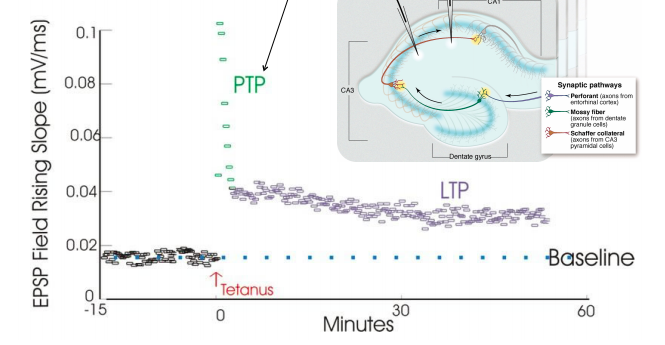
\includegraphics[width=.8\textwidth]{03_PlasticityInTheBrain/figures/pasted_image_11.png}
    \caption{Heterostatic Plasticity}
    \label{fig:syn_plas1t}
\end{figure}


LTP is measure in the hippocampus. The CA3 pathway is given a fast stimulus of (range of 50 - 200) 100 hz known as tetanus. This then leads to a stronger post tetanic potentiation caused by the accumulation of Ca in the terminals as well as LTP in the long term. If the cells are stimulated at a lower time frequency 1-10 hz LTD will occur. 




\subsubsection{LTP and LTD induction in the Hippocampus}
\subsubsection{Molecular basis of synaptic plasticity}

\begin{figure}[H]
    \centering
    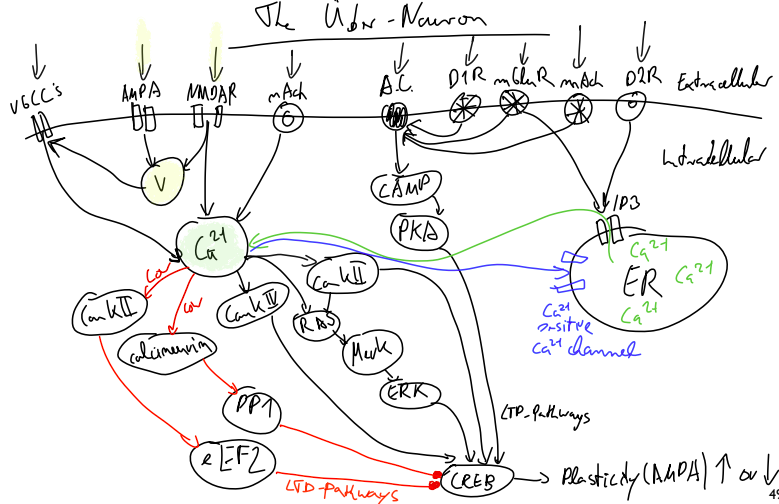
\includegraphics[width=.8\textwidth]{03_PlasticityInTheBrain/figures/pasted_image_12.png}
    \caption{}
    \label{fig:syn_plas1t}
\end{figure}

\paragraph{Intro}
Very simply LTP and LTD are dependent on CREB which controls the level of AMPA receptors in the cell. The level of AMPA receptors will determine how depolarised or hyperpolarised the cell becomes. 

\paragraph{What controls LTP and LTD:}
\begin{itemize}
    \item Creb is controlled by many pathways that are dependant on Ca ions or directly by dopamine. 
    \item Ca ion levels can increase as it enters into the cell from the external environment or released from internal stores.
\end{itemize}

\paragraph{How CA levels change:}
AMPA channel, when glutamate binds it causes depolarisation opening voltage gated Ca channels as well as NMDA channels that further depolarise the cells. 
Dopamine D2 when binds in leads to Ca2+ increase from the ER, this increased Ca leads. 

\paragraph{How CA leads to CREB:}
\begin{itemize}
    \item Positive: High levels of Ca activated Camkinse 1 and 2 that leads to increased Creb and thus ampa receptors. Dopamine activated internal cell machinery that leads to increased phosphorylation (activation) of creb these both pathways are known as the LTP pathways. 
    \item Negative: Low levels of Ca leads to Camkinse 2 and Calmodulin that reduces the phosphorylation (activation) of creb thus ampa receptors.
\end{itemize}

\paragraph{Summary}
Thus Ca is very important for LTP and LTD. Low frequency stimulation causes low Ca levels and high frequency leads to high levels.

%---------------------------
\subsection{Non-synaptic plasticity}
Researchers have artificially raised the Neuronal excitability below threshold. It leads to a greater number of firings. 

Researchers can modulate the axons with glutamate puffs and this will affect the action potential traveling along the axon. 

Researchers can modulate dendritic excitability 
If the volume is smaller the epsp will summed up leading to ap, the synapse location will also modulate the excitability nearer the soma will be more excitable as there isn’t a loss of charge.

\subsubsection{Neuronal excitability and spike generation}
\subsubsection{Axonal modulation (shunting, frequency filtering)}
\subsubsection{Alterations of dendritic excitability}


\subsection{QUIZ}
\begin{itemize}
    \item What are the differences between the weights of a deep network and the connections between biological neurons?: 
    In deep learning the weights are binary, if a neuron is activity it causes a change in the next layer.
    In biology if the action potential is modulated (axonal by myelinated and other factors) it will determine if the post neuron is activated, the dendritic epsp can be modulated before it reaches the axon hillock by summation and inhibition signals, the cell can in a refractory period or in excitability this means the effective connective between neurons can be modulated, also the inhibitory nts can modulate the epsp.
    \item Is synaptic plasticity the only mechanism that neurons can use to alter their effective connectivity?
    \item Is weight tuning by BP the only mechanism in DNNs that affect the weights?
\end{itemize}

\end{document}